\chapter{Background and Literature Review}
\label{ch:background}

\section{Breast ultrasound as an imaging modality}
Ultrasound forms images from the transmission and reception of acoustic waves. At a simplified level, the speed of a small-amplitude pressure wave in a medium is related to its bulk modulus $K$ and density $\rho$ by
\begin{equation}
c = \sqrt{\frac{K}{\rho}}.
\end{equation}
At an interface between tissues with acoustic impedances $Z_1$ and $Z_2$, the normal-incidence intensity reflection coefficient can be written as
\begin{equation}
R_I = \left(\frac{Z_2-Z_1}{Z_2+Z_1}\right)^2.
\end{equation}
Spatially varying reflection, scattering, attenuation, time-gain compensation, and scanner processing jointly determine the displayed B-mode image. The resulting pixel array is therefore not a direct tissue measurement and can vary substantially between acquisitions.

Breast ultrasound is used alongside clinical history and other imaging. Radiologists may consider features such as shape, margin, orientation, echogenicity, and posterior acoustic behaviour within the ACR BI-RADS ultrasound lexicon \citep{Mendelson2013,Stavros1995}. These descriptors provide clinical context for why geometry and local contrast matter. They do not justify inferring a BI-RADS category from this project's classifier or from its heuristic image measurements.

\section{Speckle and image variability}
Speckle arises from constructive and destructive interference among echoes from unresolved scatterers. A frequently used simplified observation model combines signal-dependent and additive components:
\begin{equation}
I(x,y)=f(x,y)\,\eta_m(x,y)+\eta_a(x,y),
\label{eq:speckle_model}
\end{equation}
where $f$ is an underlying reflectivity field, $\eta_m$ is a multiplicative term, and $\eta_a$ represents additive acquisition noise. This model is an approximation: displayed clinical images also contain beamforming, compression, filtering, and device-specific processing.

Traditional reduction methods include local-statistics filters and speckle-reducing anisotropic diffusion \citep{Lee1980,Yu2002}. More recent work evaluates learned models under perturbations to determine whether apparently strong classifiers remain stable when image quality changes \citep{Jiang2023}. Robustness must be tested on stored predictions with a specified perturbation process and seed. A visually plausible synthetic example is not by itself a performance experiment.

Filtering also changes the evidence available to a later segmentation or classification stage. Osman et al. compared filtering algorithms for breast ultrasound lesion segmentation and found that preprocessing choices can alter the resulting boundary estimate \citep{Osman2018}. Yap et al. likewise studied processed ultrasound images in relation to human perception \citep{Yap2010}. Together, these studies support treating enhancement as an experimental factor, not as an automatic improvement.

\section{Geometric preprocessing}
CNN batches usually require a common spatial size. If an image of height $H$ and width $W$ is directly resized to $H'$ by $W'$, its axis-specific scale factors are
\begin{equation}
s_y=\frac{H'}{H}, \qquad s_x=\frac{W'}{W}.
\end{equation}
When $s_x\neq s_y$, the transformation is anisotropic and changes apparent aspect ratios. An alternative is to crop a defined region, pad it to a square, and then resize it. If the square side is $d$, both axes use the same final factor $224/d$ in this project.

This geometric property is deterministic, but its effect on classification is empirical. Cropping can discard useful context; reflection padding can introduce repeated boundary structure; and mask-guided training can differ from unmasked deployment. A fair ablation must hold the partition, architecture, optimisation budget, and random seeds constant while changing only the preprocessing strategy.

\section{Contrast Limited Adaptive Histogram Equalisation}
Global histogram equalisation uses an image-wide cumulative distribution and can over-emphasise background variation. Contrast Limited Adaptive Histogram Equalisation (CLAHE) instead applies local mappings and clips histogram mass before redistribution \citep{Zuiderveld1994}. For a contextual region with histogram $h(k)$, a conceptual clipped histogram is
\begin{equation}
h_c(k)=\min(h(k),\beta)+r(k),
\end{equation}
where $\beta$ is the clip threshold and $r(k)$ distributes the clipped mass. Interpolation between neighbouring mappings reduces tile-boundary discontinuities.

The implementation in this repository applies OpenCV CLAHE to the luminance channel in LAB colour space, with a clip limit of 2.0 and a $16\times16$ tile grid. This is a documented configuration choice, not evidence that CLAHE improves discrimination. Its effect requires a controlled ablation and should include both predictive and image-quality analysis.

\section{Convolutional representation learning}
CNNs learn filters through repeated convolution, non-linearity, and aggregation. For an activation tensor $\mathbf{X}^{(l-1)}$, a layer can be represented schematically as
\begin{equation}
\mathbf{X}^{(l)}=\sigma\!\left(\mathbf{W}^{(l)}*\mathbf{X}^{(l-1)}+\mathbf{b}^{(l)}\right).
\end{equation}
Medical-image datasets are often much smaller than general computer-vision corpora, so transfer learning is commonly used to initialise useful low- and mid-level features \citep{Litjens2017}.

\subsection{ResNet-50}
Residual networks learn a residual function around an identity path,
\begin{equation}
\mathbf{y}=\mathcal{F}(\mathbf{x},\{\mathbf{W}_i\})+\mathbf{x},
\end{equation}
which supports optimisation of deeper architectures \citep{He2016}. In this project, the original classification layer is replaced by dropout and a two-output linear layer.

\subsection{EfficientNet-B0}
EfficientNet uses coordinated scaling of network depth, width, and input resolution, with the B0 model serving as the baseline architecture \citep{Tan2019}. Its mobile inverted bottleneck blocks include squeeze-and-excitation operations that reweight channels \citep{Hu2018}. The project replaces the classifier with dropout and a two-output linear layer.

\subsection{Custom CNN baseline}
The custom model provides a compact, from-scratch baseline with four convolutional stages, batch normalisation, ReLU activations, max pooling, adaptive average pooling, dropout, and a two-output layer. It helps distinguish the contribution of transfer learning from that of the surrounding pipeline, but a fair comparison requires equivalent split integrity and a predeclared tuning budget.

\section{Outputs, confidence, and explanation}
The two logits are converted to a mutually exclusive probability vector using softmax:
\begin{equation}
p(y=c\mid\mathbf{x})=\frac{\exp(z_c)}{\sum_{j=1}^{K}\exp(z_j)}.
\end{equation}
Softmax normalisation does not guarantee calibration. Neural networks can be overconfident, so a displayed score must not be interpreted as diagnostic certainty \citep{Guo2017}. Calibration should be evaluated on an independent validation design if the model is developed further.

Grad-CAM uses gradients flowing into a convolutional layer to form a coarse localisation map \citep{Selvaraju2017}. Such maps can support debugging and hypothesis generation, but they neither prove causal reasoning nor validate clinical relevance. This project labels them as research visualisations.

Breast ultrasound research by Yap and colleagues also shows how the task has moved from handcrafted lesion localisation and conventional classification towards end-to-end and attention-based learning. Early work addressed initial lesion detection and compared classification pipelines \citep{Yap2008,Yap2009}. Later studies evaluated convolutional detection, end-to-end lesion recognition, and region-of-interest localisation \citep{Yap2018,Yap2019,Yap2020ROI}. AAU-Net extended this line of work to adaptive attention for lesion segmentation \citep{Chen2023}. These papers cover different tasks, so their reported scores are not interchangeable with the binary image classification result in this dissertation. Their main contribution here is methodological: localisation, preprocessing, split design, and evaluation must be specified together.

\section{Review of public breast ultrasound datasets}
\label{sec:dataset_review}

Public breast ultrasound datasets differ in acquisition, annotation, reference standard, lesion mix, and file organisation. These differences affect what a model can learn and how its results should be interpreted. BUS-Set brought OASBUD, RODTOOK, UDIAT, and BUSI into a common segmentation benchmark and showed the practical value of published folds and coordinated evaluation \citep{Thomas2023}. Bristow and Yap later reviewed those sources alongside BrEaST while studying the effect of resizing on classification \citep{Bristow2026}. Table~\ref{tab:public_dataset_review} summarises the five sources considered in that review. The counts are for the curated single-lesion benign and malignant subset in their manuscript; the local cohort used in this dissertation differs.

\begin{table}[htbp]
\centering
\caption{Public breast ultrasound datasets reviewed by Bristow and Yap. Counts refer to their curated classification subset \citep{Bristow2026}.}
\label{tab:public_dataset_review}
\small
\begin{tabularx}{\textwidth}{@{}p{0.16\textwidth}p{0.14\textwidth}p{0.14\textwidth}X@{}}
\toprule
\textbf{Dataset} & \textbf{Country} & \textbf{\shortstack[l]{Curated\\images}} & \textbf{Evidence and curation considerations} \\
\midrule
OASBUD & Poland & 199 & Raw radio-frequency acquisitions require B-mode reconstruction. Lesion labels include biopsy and follow-up evidence, and related views require subject grouping \citep{Piotrzkowska2017}. \\
RODTOOK & Thailand & 165 & The source study contains 180 images and radiologist-drawn references for malignant tumours, fibroadenomas, and cysts. Scanner overlays and duplicate handling require curation \citep{Rodtook2018,Bristow2026}. \\
UDIAT & Spain & 159 & The public set contains a small benign and malignant cohort with radiologist contours and one scanner source. It has been used for detection and segmentation research \citep{Yap2018,Thomas2023}. \\
BUSI & Egypt & 332 & The original release contains 780 normal, benign, and malignant images with masks \citep{AlDhabyani2020}. Published correspondence identifies duplicates, conflicting labels, and non-breast or overlay cases that require explicit handling \citep{Pawlowska2023}. \\
BrEaST & Poland & 252 & The source contains 256 patient scans, manual lesion annotations, BI-RADS descriptors, and outcomes confirmed by biopsy or follow-up. Images came from several radiologists and scanners \citep{Pawlowska2024}. \\
\bottomrule
\end{tabularx}
\end{table}

\subsection{Ground truth, image quality, and representation}

OASBUD and BrEaST provide the clearest route from image to patient-level evidence among the datasets available to this project. OASBUD includes raw signal data, reconstructed images, lesion masks, and subject identifiers. Its reconstructed B-mode images are visibly lower in resolution and noisier than many conventional exported scans. BrEaST has manual annotations and detailed patient, image, and tumour labels; the source article reports 154 benign lesions, 98 malignancies, and four normal cases from 256 patients \citep{Pawlowska2024}. The two datasets therefore differ enough in appearance to expose some acquisition sensitivity while retaining identifiers needed for group-aware splitting.

RODTOOK and UDIAT remain useful public resources, especially for segmentation and detection comparison \citep{Rodtook2018,Yap2018,Thomas2023}. They were absent from the supplied project data. Adding them would have required a new acquisition, licensing, curation, and audit cycle after the experimental protocol had been defined. They remain suitable candidates for a later external evaluation.

BUSI was available locally, but it was not suitable for the validated experiment in its present form. Its files had been renamed to generated sample identifiers and reduced to square derivatives before this revision. The original release contains masks and three diagnostic categories \citep{AlDhabyani2020}, while later correspondence identifies duplicate images, label conflicts, non-breast content, and overlays that require case-level curation \citep{Pawlowska2023}. Renaming broke the link needed to repeat those published checks. It also removed the evidence needed to keep every image from one patient in a single partition. A new random split of the derivative files could therefore place related or duplicated observations on both sides of the train-test boundary.

The decision to exclude BUSI is based on study validity rather than convenience. Its additional images would increase the apparent sample size, but they would also introduce a source whose identity, curation decisions, and patient independence cannot be reconstructed from the files now held in the project. Mixing that source into the test set would make the denominator larger without making the estimate more trustworthy. BUSI remains a valuable public dataset when obtained from the original release and curated with a versioned manifest. This dissertation makes no claim about its intrinsic clinical quality; it excludes only the local derivative copy.

Image-level variation is visible before modelling. Figure~\ref{fig:dataset_quality_examples} compares representative local samples and their recorded pixel dimensions. OASBUD reconstruction produces a square, grainier appearance, whereas BrEaST contains sharper exported scans with variable aspect ratios. The local BUSI files have already been reduced to square images and show repeated banding, so they cannot be treated as untouched examples of the published BUSI release. The plate records these visible differences without assigning a quality score.

\begin{figure}[htbp]
    \centering
    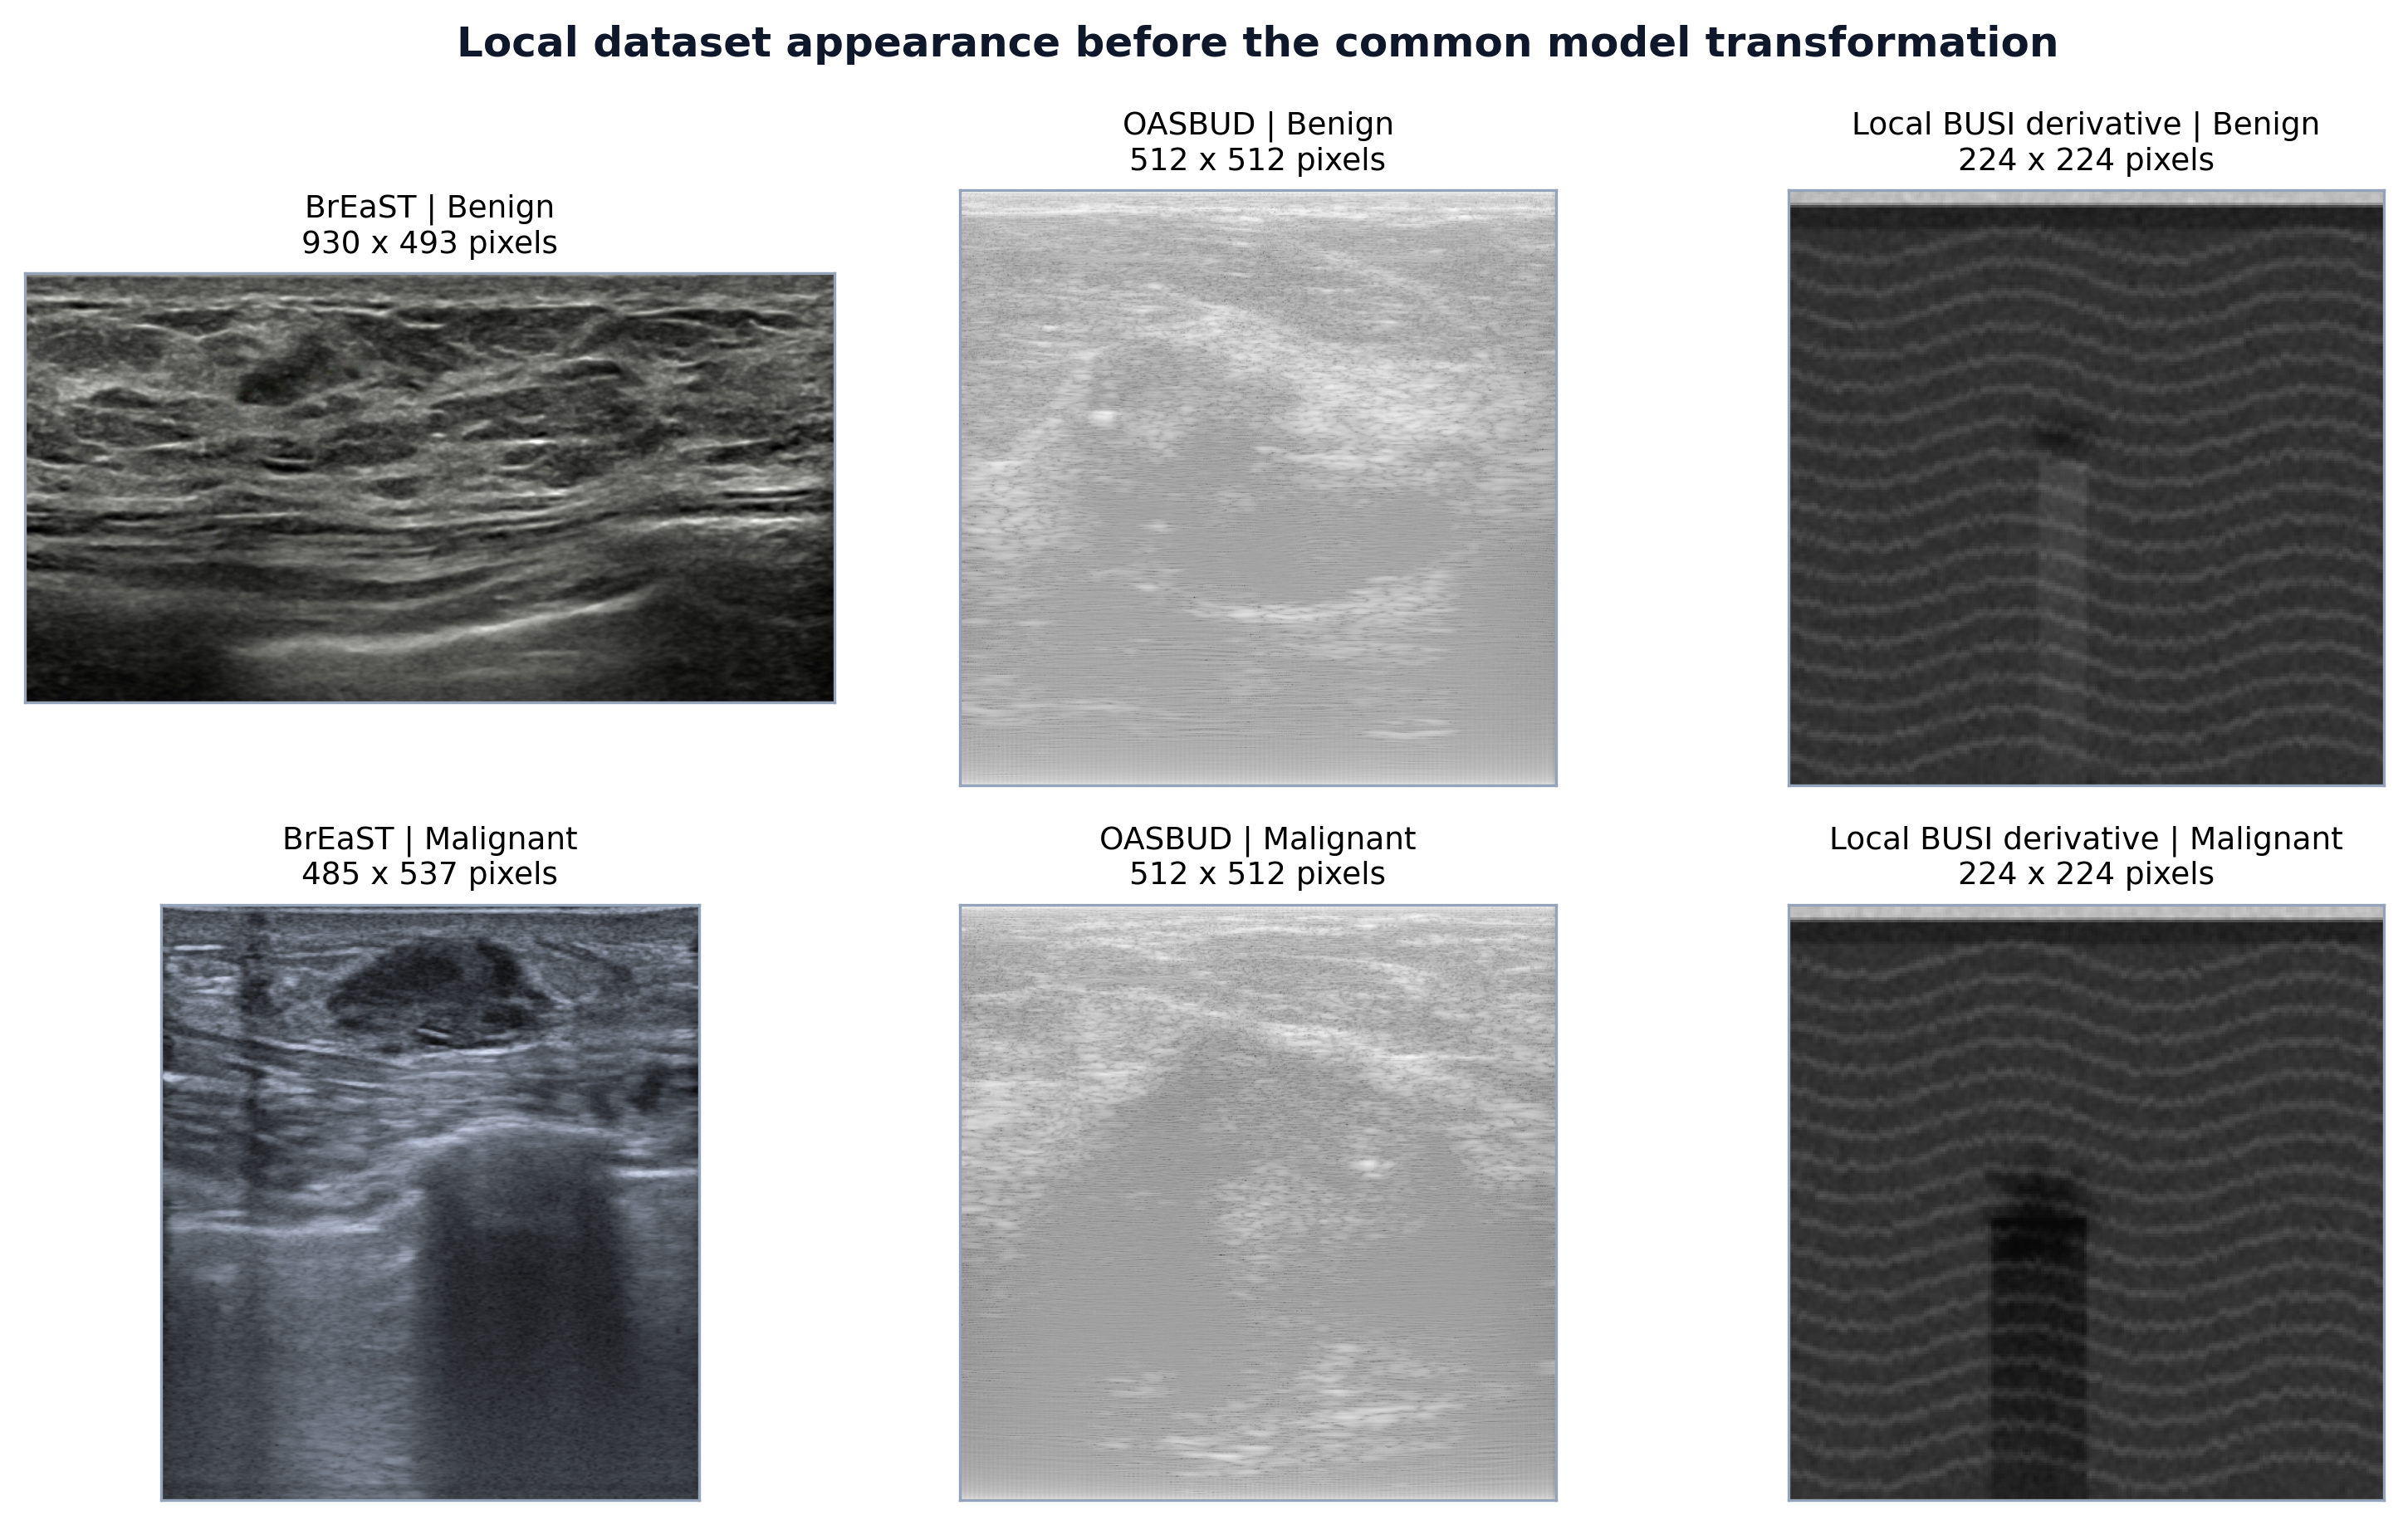
\includegraphics[width=0.96\textwidth]{figures/fig9_dataset_quality_examples.png}
    \caption{Representative benign and malignant images from the local BrEaST, OASBUD, and BUSI-derived folders. Each image retains its display aspect ratio. The BUSI panels show the processed local derivative rather than the original public release, which is why those files are excluded from validated evaluation.}
    \label{fig:dataset_quality_examples}
\end{figure}

\subsection{Justification for the selected research cohort}

The validated experiment uses OASBUD and BrEaST for four practical reasons. First, both retain subject identifiers that support deterministic grouping and a direct cross-partition audit. Second, both provide lesion annotations that the common region-of-interest pipeline can discover. Third, their labels have documented biopsy or follow-up support, although the proportion and form of verification differ across benign cases \citep{Piotrzkowska2017,Pawlowska2024,Bristow2026}. Fourth, their contrasting image appearance provides a more informative local test than training and evaluating on one source alone.

This choice also has limitations. Both datasets originate in Poland, and the local audited test set contains only 62 images. The study therefore does not measure geographic generalisation, performance across the full range of scanners, or clinical prevalence. RODTOOK, UDIAT, or an independently obtained original BUSI release with verified provenance could support a later external study. That later protocol should freeze patient-level manifests before model selection and report results separately for each source rather than presenting a pooled score alone.

The review supports the evidence boundary adopted in this dissertation. Published breast ultrasound studies remain heterogeneous in population, reference standard, threshold, and validation design. A 2024 systematic review found insufficient evidence that deep learning systems outperform or consistently assist human readers in clinical breast ultrasound and called for more standardised, multicentre evaluation \citep{Dan2024}. Earlier observer research also showed that agreement varies by sonographic feature and case difficulty \citep{Shimamoto1998}. These findings support cautious reporting of the present local-cohort result.

\section{Literature synthesis and research gap}
The literature establishes several relevant components: public breast-ultrasound datasets and coordinated benchmarks \citep{AlDhabyani2020,Piotrzkowska2017,Thomas2023,Pawlowska2024}; lesion localisation and classification from conventional methods through end-to-end convolutional systems \citep{Yap2008,Yap2009,Yap2018,Yap2019,Yap2020ROI,Cheng2016,Zeimarani2020}; efficient and residual transfer-learning architectures \citep{He2016,Tan2019}; image enhancement and filtering \citep{Zuiderveld1994,Yap2010,Osman2018}; attention-based segmentation \citep{Chen2023}; and perturbation-based robustness testing \citep{Jiang2023}. Sonographic appearance can also vary with lesion size and subtype, which makes a narrowly sampled image collection a weak basis for broad clinical claims \citep{Yoon2018}. The gap addressed here is practical integration with an explicit evidence boundary. A classifier, dashboard, and polished report can appear complete while still lacking the provenance needed to justify its headline numbers.

Accordingly, this dissertation treats data auditability as part of the modelling method. It implements the full software path, reports the current executable output as provisional, and defines the group-aware experiment required before comparative or clinical conclusions can be drawn.

\section{Image formation and within-subject variation}
In practice, the displayed image contains several transformations between the acoustic interaction and the pixel values saved to disk. Beamforming combines received signals; envelope detection converts oscillatory information into an intensity representation; log compression maps a large dynamic range into a displayable range; and post-processing may smooth, sharpen, or suppress parts of the signal. The exact sequence is device-dependent and is rarely recoverable from a public PNG file. A learning system therefore observes a measurement product rather than a neutral photograph of anatomy.

This has two consequences for the present study. First, a network may exploit acquisition cues that correlate with a label in one collection. Second, a preprocessing operation that makes an image look clearer to a person may remove a cue that the network used, or may amplify a nuisance pattern. The appropriate response is not to assume that enhancement is beneficial. It is to record the operation, compare it under controlled conditions, and inspect errors with the same transformation used at inference.

Image variability also exists within a subject. A lesion may be captured at different angles, depths, or compression states. These views are related observations, not independent samples. If one view is placed in training and another in testing, the test score estimates recognition of a familiar subject distribution more than recognition of a new patient. This is why a subject-level grouping rule is part of the experimental design rather than a post-hoc data-cleaning step.

\section{Practical implications of preprocessing choices}
The choice of crop is as important as the choice of resize. A tight lesion crop can increase the proportion of pixels occupied by the region of interest, but it can remove posterior shadowing, surrounding tissue, or the probe-related context that a radiologist would use. A wide crop retains context but makes the lesion smaller after resizing. When a mask is available, the margin around the bounding box is therefore a modelling decision rather than a neutral technical detail. The fixed margin used here is an inspectable rule, not an optimised clinical parameter.

Padding introduces a different prior. Reflection padding copies local boundary structure, reducing the hard edge produced by constant padding, but it can also create a repeated texture that was not acquired by the scanner. Centre cropping avoids invented borders but may remove an off-centre lesion. Direct resizing preserves every pixel but changes shape. These trade-offs can be described mathematically, yet their clinical relevance remains empirical. A good report should show representative transformations and retain the original-to-processed mapping so that an apparent improvement can be traced back to a concrete change in the input.

CLAHE also changes the distribution seen by a pretrained backbone. ImageNet weights were learned from natural images with a particular range of colour and local contrast. Applying a luminance transformation may make lesion boundaries easier to inspect, but it can move the input away from the statistics assumed by the initial filters. This is one reason to keep the operation configurable rather than baking it into a hidden data-export step. It allows checkpoint metadata to state whether the model saw raw or enhanced input.

\section{Transfer learning under small-sample uncertainty}
Transfer learning is not a guarantee of suitability. The source and target domains differ in colour, texture, scale, and semantic structure. Early convolutional filters may still provide useful edge and frequency responses, whereas later layers can encode object categories that are irrelevant to ultrasound. Fine-tuning all layers on a small cohort may overfit; freezing too many layers may leave a domain mismatch unresolved. A defensible experiment should state which layers are trainable, whether pretrained weights were downloaded at run time, and whether the same schedule was applied to every comparator.

The small-data setting creates a second issue: the variance of a metric can be as important as its point estimate. With only a few dozen test images, one changed prediction moves accuracy by more than one percentage point. A ranking of three architectures on one split can therefore be unstable. The comparison is useful as a baseline and as a source of hypotheses, while a larger frozen cohort is needed for a firmer ranking.

\section{Interpreting confidence and explanation}
The interface uses an abstention threshold as a presentation choice. When the maximum class probability is below the configured threshold, the API returns an ``UNCERTAIN'' display prediction while preserving the underlying model prediction and probabilities. Abstention does not calibrate the model or make it safe. It prevents low-margin outputs from being presented as decisive labels. A future study should select the threshold on validation data, report coverage alongside selective risk, and test whether abstention removes ambiguous cases across datasets rather than only within one split.

Explanations should be read in the same cautious way. Grad-CAM highlights the sensitivity of a selected feature map under a particular forward and backward pass. It does not identify a lesion boundary, establish that the highlighted pixels caused the decision, or replace a reader study. Useful checks include overlaying maps on images from both classes, measuring stability under small transformations, and comparing maps for correct and incorrect predictions. These checks can reveal shortcut learning, but a visually plausible overlay remains a debugging aid rather than a clinical explanation.

\section{Provenance as part of the literature gap}
Provenance includes more than a citation to a dataset paper. A repository should record the precise archive or release used, the local transformation applied to filenames, the licence terms, and any excluded files. If a file is renamed, the original identifier should be retained in a manifest rather than discarded. If masks are copied beside images, their relationship should be checked programmatically. If a label is collapsed, the mapping should be written down before training. These details are easy to omit because they do not appear in a model summary, yet they determine whether another researcher can reconstruct the cohort.

Evaluation design should distinguish development decisions from final measurement. Hyperparameters, preprocessing choices, and checkpoints are selected using development data. The test set is then used once to estimate performance under the predeclared protocol. Repeatedly inspecting test predictions and adjusting the model creates a hidden validation loop. On a small dataset this leakage can be subtle: a researcher may remember a difficult image, change a crop rule, and rerun the test without recording the decision. A frozen manifest and generated artefacts provide a simple defence against that drift.

\section{From clinical descriptors to pixels}
Clinical ultrasound descriptors are not pixel labels. Shape, orientation, margin, echogenicity, and posterior features are interpreted together and in relation to patient history. A classifier that receives only a cropped image has no explicit access to that history and may not observe every descriptor reliably. Pixel learning can still answer a narrower question: whether the image representation contains information correlated with the supplied class label.

The distinction also affects explanation. A saliency map that highlights a margin-like region may be consistent with a clinical description, but consistency is not validation. A map that highlights a ruler, annotation, or dark border may reveal a shortcut. Human review should therefore compare explanations with acquisition context and, where possible, with independent lesion annotations. The correct conclusion may be that a model is using an artefact, even if its numerical score is high.

\section{Class imbalance and decision thresholds}
Binary classification is often presented as if the two errors have equal consequences. In practice, the preferred operating point depends on the purpose of the system. A screening aid may prioritise sensitivity, whereas a triage tool may need a different balance of false positives and false negatives. The present project reports threshold-free ranking through ROC-AUC and thresholded predictions at the evaluator's default rule, but it does not select a clinical operating point.

The current report includes a precision-recall curve from the stored test probabilities. This view becomes especially important if the malignant class is less frequent in an external cohort. It should always be read with the class count and uncertainty because a curve can look persuasive while being supported by few positive cases. This is another reason to retain the per-image prediction table.

\section{Reproducible reporting in medical imaging}
Good reporting involves more than adding decimal places. It requires naming the unit of split, describing preprocessing, identifying the source of labels, and making exclusions visible. A reader should be able to answer which images were used, which were withheld, and whether any subject appeared in more than one partition. The audit and manifest in this project address those questions.

The literature review therefore supports a restrained conclusion. CNNs, transfer learning, CLAHE, and saliency methods are all reasonable tools for exploration, but none removes the need for provenance. The most transferable lesson is procedural: a result becomes more credible when a second person can reproduce it from the stored configuration and see where uncertainty enters the chain.
